\section{迁移 CUDA 代码}
本书的许多读者可能遇到过用 CUDA 编写的数据并行代码。 
有些读者甚至可能是 CUDA 专家! 在本章中,我们将描述 CUDA 和 SYCL 之间的一些相似之处、一些差异,
以及帮助使用 SYCL 将 CUDA 代码有效且高效地迁移到 C++ 的有用工具和技术。

\subsection{CUDA 和 SYCL 之间的设计差异}
在我们深入了解细节之前,首先确定 CUDA 和 SYCL 之间的关键设计差异具有指导意义。 
这可以提供有用的背景来说明为什么存在一些差异,了解哪些差异可能会随着时间的推移而消失以及哪些差异可能会保留。

\subsubsection{多个目标与单个设备目标}
CUDA 和 SYCL 之间最大的设计差异之一是它们设计支持的设备范围。 
CUDA 旨在支持来自单一设备供应商的 GPU 设备,因此大多数 CUDA 设备看起来相对相似。 
例如,所有 CUDA 设备当前都包含纹理采样硬件,并且所有 CUDA 设备当前都支持相同的最大Work-Groups大小。 
这降低了复杂性,但也减少了 CUDA 应用程序可以运行的位置。

相比之下,SYCL 旨在支持多种异构加速器,包括来自不同设备供应商的不同设备。 
这种灵活性使 SYCL 程序可以自由地利用现代异构系统中的计算资源; 
然而,这种灵活性的代价并不大。 例如,作为 SYCL 程序员,我们可能需要枚举系统中的设备,
检查它们的属性,并选择最适合运行程序的不同部分的设备。

当然,如果我们的 SYCL 程序不打算利用系统中的所有计算资源,
则可以使用各种快捷方式来减少代码冗长,例如标准设备选择器。 
图 21-1 显示了一个基本 SYCL 示例,该示例使用由 SYCL 实现选择的默认设备队列。

\begin{figure}[H]
	\centering
	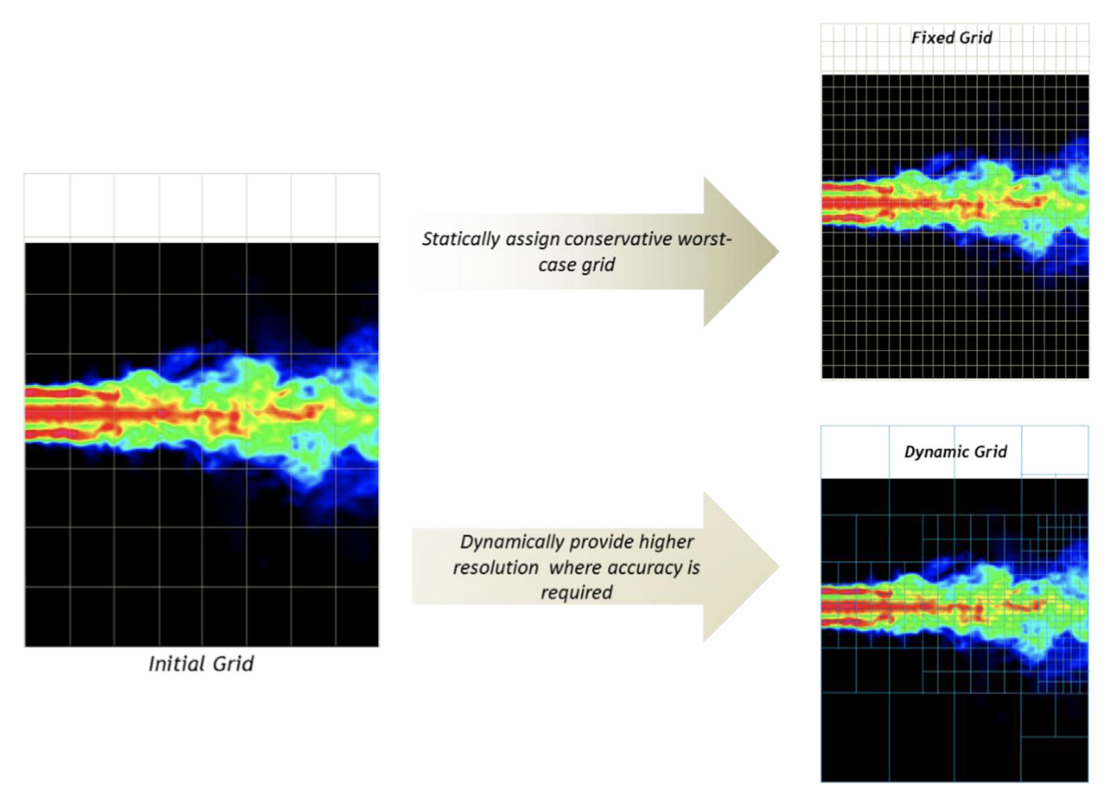
\includegraphics[width=0.9\textwidth]{figs/F21.1.png}
	\caption{\textit{在默认 SYCL 设备上运行Kernel }}
\end{figure}

此 SYCL 代码与等效的 CUDA 代码非常相似,如图 21-2 所示。

\begin{figure}[H]
	\centering
	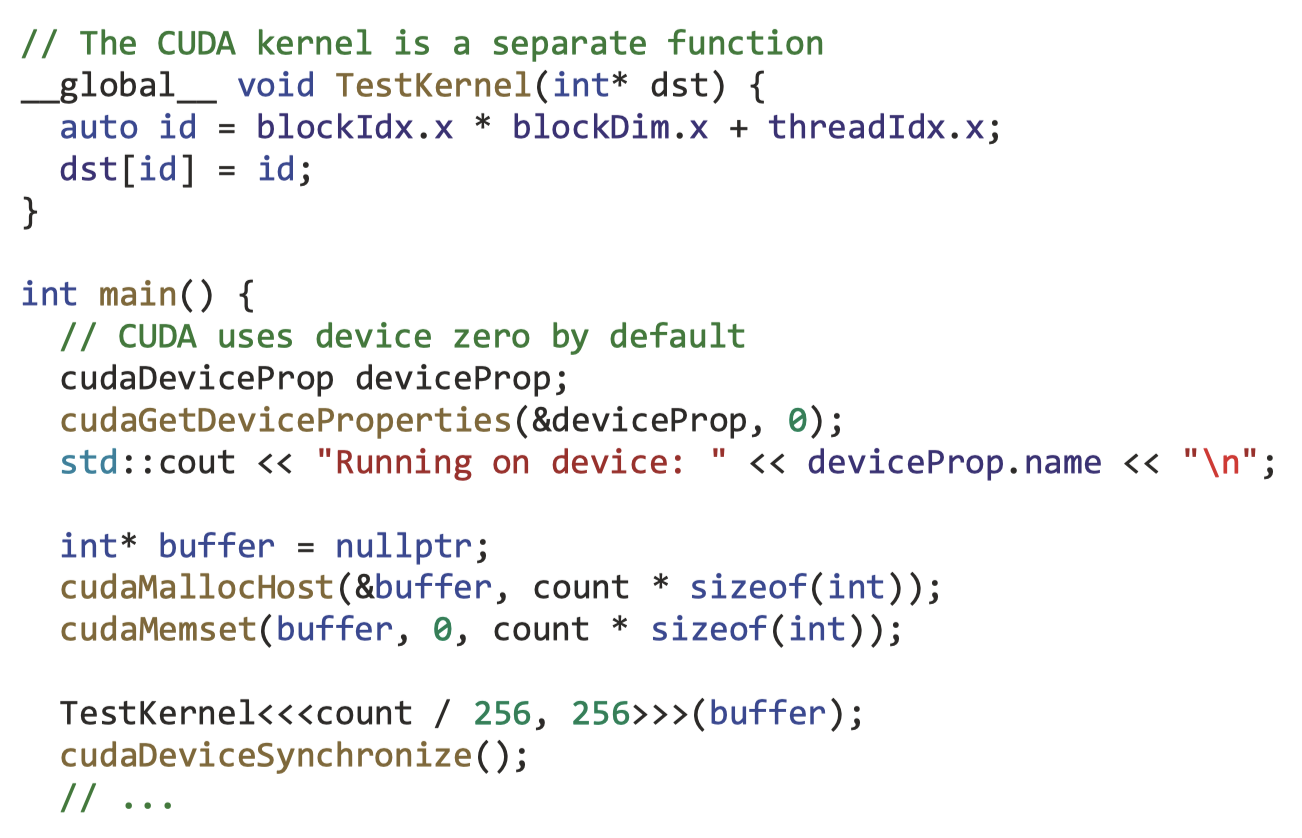
\includegraphics[width=0.9\textwidth]{figs/F21.2.png}
	\caption{\textit{在默认 CUDA 设备上运行Kernel }}
\end{figure}

现实世界的 SYCL 代码通常更复杂。 
例如,许多 SYCL 应用程序将通过搜索特定设备特征(请参阅第 12 章)来枚举
并选择要运行的特定设备或设备组合(请参阅第 2 章)。 
然而,当不需要或不需要这种复杂性时,存在简洁的选项,并且 SYCL 经过精心设计,可以在需要时支持额外的复杂性。

\subsubsection{对齐 C++ 与扩展 C++}
CUDA 和 SYCL 之间的另一个重要设计差异是它们如何与其他编程语言(尤其是 C++)交互。 
SYCL 代码是标准 C++ 代码,没有任何语言扩展。 
通过学习阅读、理解和编写 C++ 代码,我们也能够阅读和理解 SYCL 代码。 
同样,如果编译器可以解析 C++ 代码,它也可以解析 SYCL 代码。

CUDA 做出了不同的决定。 相反,CUDA 通过添加新关键字和特殊语法来执行Kernel来扩展 C++。 
有时,语言扩展可以更简洁,但它们也是一种需要学习和记住的语法,
并且语言扩展意味着 CUDA 代码只能由支持 CUDA 的编译器编译。

要在实践中看到这种设计差异,请注意图 21-1 中的 SYCL 示例如何使用标准 C++ lambda 表达式来表示Kernel代码,
并使用标准 C++ 函数调用来提交Kernel执行。 
图 21-2 中的 CUDA 示例使用特殊的 \_\_global\_\_ 关键字来标识Kernel代码,
并使用特殊的 < < < > > > 语法来提交Kernel执行。

\subsection{CUDA 和 SYCL 之间的术语差异}
现在我们了解了 SYCL 和 CUDA 之间的一些关键设计差异,我们几乎准备好开始检查具体的相似点和差异。 
不过,我们首先需要了解一点背景知识:因为 CUDA 和 SYCL 经常对相似的概念使用不同的术语,
所以我们需要一个解码器,以便我们可以有意义地比较这两个 API,如图 21-3 中的摘要所示。

\begin{figure}[H]
	\centering
	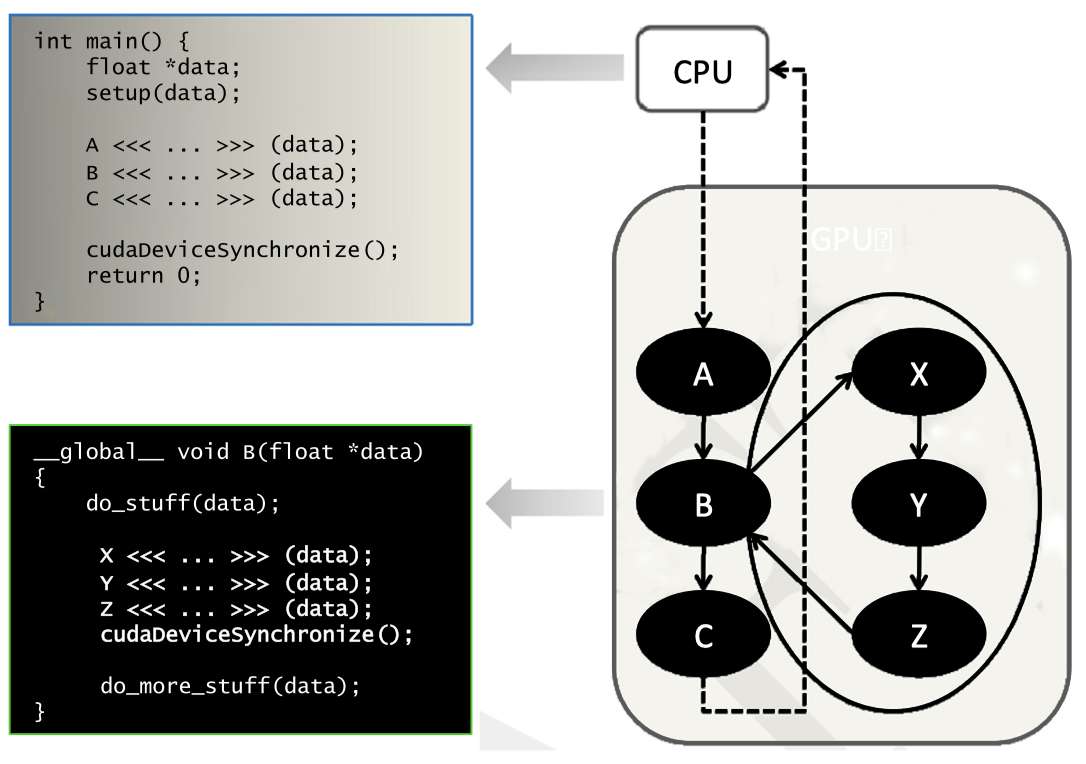
\includegraphics[width=0.9\textwidth]{figs/F21.3.png}
	\caption{\textit{CUDA 和 SYCL 解码器环 }}
\end{figure}

与本书其余部分一致使用 SYCL 术语不同,本章可以互换使用 CUDA 术语和 SYCL 术语。

\subsection{共同点和不同点}
本节介绍 SYCL 和 CUDA 之间的一些语法和行为相似之处以及 SYCL 和 CUDA 的不同之处。

\subsubsection{执行模型}
从根本上来说,SYCL 和 CUDA 都使用第 4 章中介绍并在本书中描述的相同数据并行Kernel执行模型。 
术语可能略有不同,例如,SYCL 指的是 ND 范围,CUDA 指的是网格,
但我们可以使用图 21-3 中的解码器环将关键概念从 SYCL 转换为 CUDA,反之亦然。

\paragraph{有序队列与无序队列}

尽管执行模型有许多相似之处,但确实存在一些差异。 一个区别是 CUDA 流是无条件有序的。 
这意味着提交到 CUDA 流的任何Kernel或内存操作必须在下一个提交的Kernel或内存复制操作开始之前完成。 
相反,SYCL 队列默认是无序的,
但可以选择在创建 SYCL 队列时通过传递 in\_order 队列属性来按顺序排列(请参阅第 8 章)。

有序 CUDA 流更简单,因为它不需要显式调度或依赖性管理。 
这种简单性意味着 CUDA 应用程序通常不使用访问器或 dependent\_on 等机制来对流中的操作进行排序。 
不过,有序语义也限制了执行,并且不提供任何在单个流中重叠执行两个命令的机会。 
由于 CUDA 应用程序不能重叠执行单个流中的两个命令,
因此当 CUDA 应用程序想要(可能)同时执行命令时,它将把命令提交到不同的 CUDA 流,
因为不同 CUDA 流中的命令可能会同时执行。

这种提交到多个有序队列以同时执行Kernel或内存操作的相同模式也适用于 SYCL,
并且许多 SYCL 实现和 SYCL 设备都经过优化来处理这种情况。 
不过,无序 SYCL 队列提供了一种替代机制,可以仅与单个队列重叠执行,
并且许多 SYCL 实现和 SYCL 设备也经过优化以处理这种情况。

最终,是否使用多个有序 SYCL 队列或更少的无序 SYCL 队列取决于个人喜好和编程风格,
我们可以选择对我们的 SYCL 程序最有意义的选项。 
本章中的 SYCL 示例创建有序 SYCL 队列,以尽可能接近等效的 CUDA 示例。

\paragraph{连续维度}

可能让新手和专家 CUDA 程序员感到困惑的另一个区别涉及多维 SYCL 范围或 CUDA 网格:
SYCL 将其约定与标准 C++ 中的多维数组对齐,因此最后一个维度是连续维度,也称为单位跨度维度或 移动最快的维度。 
相反,CUDA 与图形约定保持一致,因此第一个维度是连续维度。 
由于这种差异,与等效的 CUDA 代码相比,多维 SYCL 范围将出现转置,
并且 SYCL id 的最高维度将对应于可比较 CUDA 内置变量的 x 分量,而不是最低维度。

\begin{figure}[H]
	\centering
	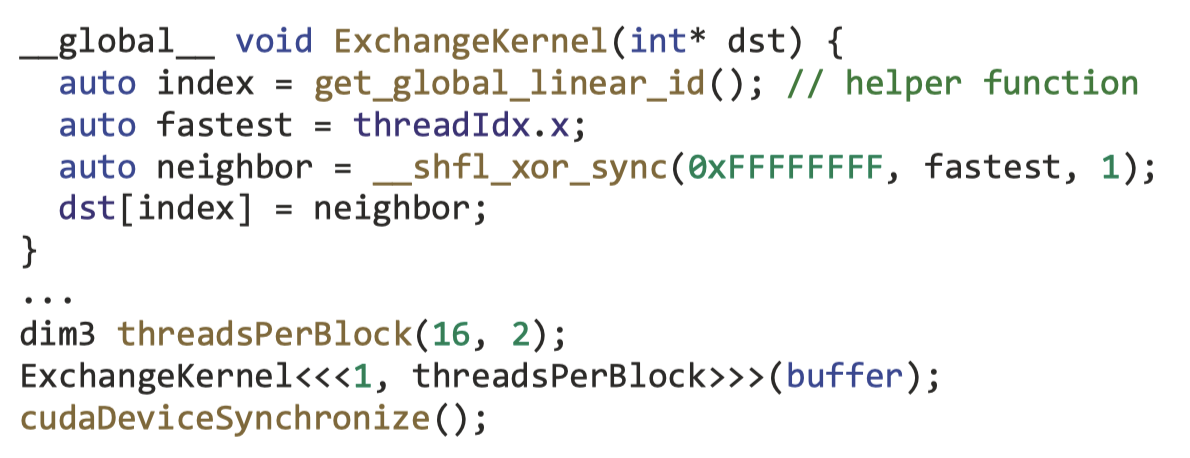
\includegraphics[width=0.9\textwidth]{figs/F21.4.png}
	\caption{\textit{x-component 是 CUDA 中的连续维度 }}
\end{figure}

为了演示这种差异,请考虑图 21-4 中的 CUDA 示例。 
在此示例中,每个 CUDA 线程与其邻居交换其 threadIdx.x 值。 
由于 x 组件是 CUDA 中移动最快的组件,因此我们不期望 CUDA 线程的值与其相邻线程的值匹配。

\begin{figure}[H]
	\centering
	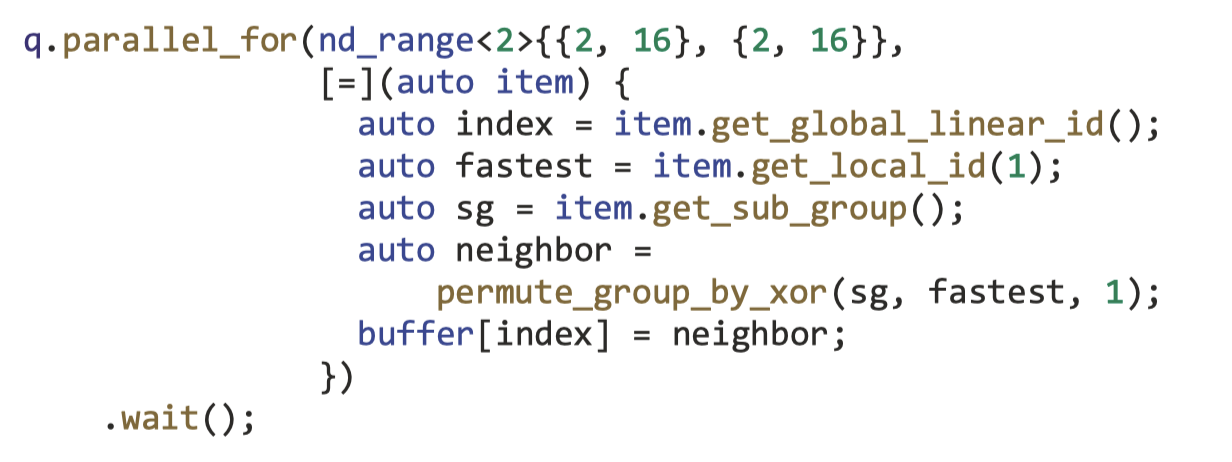
\includegraphics[width=0.9\textwidth]{figs/F21.5.png}
	\caption{\textit{最后一个维度是 SYCL 中的连续维度 }}
\end{figure}

等效的 SYCL 示例如图 21-5 所示。 请注意,在 SYCL 示例中,ND 范围是 \{2, 16\},
而不是 CUDA 示例中的 (16, 2),因此并行索引空间似乎已转置。 
SYCL 示例还将 ND 范围描述为 \{2, 16\} 全局范围,分为大小为 \{2, 16\} 的Work-Groups,
而 CUDA 示例描述了一个块的网格,每个块有 (16, 2) 个 CUDA 线程。

此外,请注意,每个 SYCL Work-Items都会与其邻居交换其 item.get\_local\_id(1)
(不是 item.get\_local\_id(0)!)的值,因为最后一个维度是 SYCL 中移动最快的组件。 
在此 SYCL 示例中,我们也不期望 SYCL Work-Items的值与其相邻Work-Items的值相匹配。

\paragraph{Sub-Groups尺寸(变形尺寸)}

如果仔细查看这些示例,我们还可以发现更多差异,特别是与用于与邻居交换数据的函数相关的差异。

CUDA 示例使用函数 \_\_shfl\_xor\_sync(0xFFFFFFFF,fastest,1) 与邻居交换数据。 
对于此函数,第一个参数 0xFFFFFFFF 是一个位域掩码,指示参与调用的 CUDA 线程集。 
对于 CUDA 设备,32 位掩码就足够了,因为当前所有 CUDA 设备的扭曲大小均为 32。

SYCL 示例使用函数 permute\_group\_by\_xor(sg,fastest,1) 与其邻居交换数据。 
对于此函数,第一个参数描述参与调用的Work-Items集。 在这种情况下,sg 代表整个Sub-Groups。 
由于Work-Items集是由组对象而不是位域掩码指定的,因此它可以表示任意大小的集。 
这种灵活性是可取的,因为对于某些 SYCL 设备,Sub-Groups大小可能小于或大于 32。

\begin{figure}[H]
	\centering
	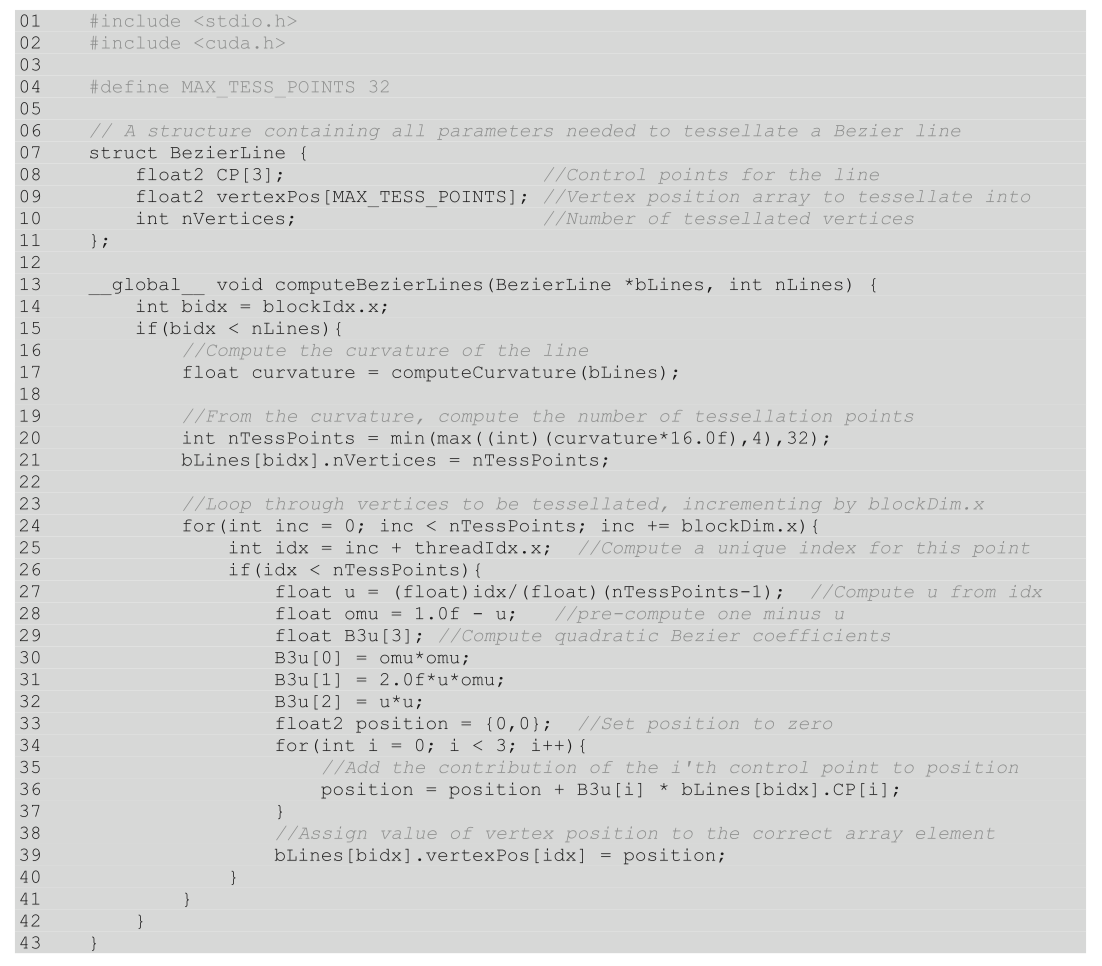
\includegraphics[width=0.9\textwidth]{figs/F21.6.png}
	\caption{\textit{与CUDA合作小组交换数据 }}
\end{figure}

在这种特定情况下,可以重写 CUDA 示例以使用更现代的 CUDA 协作组语法,
而不是旧的 \_\_shfl\_xor\_sync 语法。 等效的 CUDA 协作组如图 21-6 所示。 
该版本看起来更像 SYCL Kernel,是 CUDA 和 SYCL 2020 的后续版本如何变得更加紧密的一个很好的例子。

\paragraph{前进进度保证}

如果我们仔细观察图 21-4 和 21-5 中的示例,我们会发现另一个差异,尽管这种差异更为微妙。 
同样,差异与用于与邻居交换数据的 \_\_shfl\_xor\_sync 函数有关,
在这种情况下,差异由函数上的 \_sync 后缀暗示。 
\_sync 后缀表示该函数正在同步 CUDA 线程,尽管这自然会导致我们问,
为什么在调用该函数之前 CUDA 线程可能首先不同步?

在第 15 章和第 16 章中,我们为在 CPU 或 GPU 上执行的数据并行Kernel开发了一个心智模型,
其中使用 SIMD 指令同步处理一组Work-Items。 
虽然这对于许多供应商的 CPU 和 GPU 来说是一个有用的心智模型,
但它并不是使用 SYCL 或 CUDA 执行数据并行Kernel的唯一方法,
并且这种心智模型崩溃的情况之一是对于支持的较新 CUDA 设备 称为独立线程调度的功能。

对于具有独立线程调度的 CUDA 设备,各个 CUDA 线程独立进行,而不是作为一个组进行。 
这些额外的前向进度保证使代码模式能够在 CUDA 设备上安全执行,
而如果没有更强的前向进度保证,这些代码模式可能无法在 SYCL 设备上正确执行。 
CUDA 中添加了 \_\_shfl\_xor\_sync 函数上的 \_sync 后缀,
以明确指示该函数需要同步并指定使用 32 位掩码进行同步的 CUDA 线程。

前向进度保证是 SYCL 社区中的一个活跃主题,并且 SYCL 的未来版本很可能会添加查询以确定设备的前向进度功能,
以及用于指定Kernel的前向进度要求的属性。 不过,目前我们应该意识到,由于独立的线程调度,
从 CUDA 移植的语法正确的 SYCL 程序可能无法在所有 SYCL 设备上正确执行。

\paragraph{Barrier}

我们应该注意的最后一个微妙的执行模型差异涉及 CUDA 的 \_\_syncthreads 函数
与 SYCL group\_barrier 等效函数的比较。 
CUDA 的 \_\_syncthreads 函数同步线程块中的所有未退出的 CUDA 线程,
而 SYCL group\_barrier 函数同步Work-Groups中的所有Work-Items。 
这意味着,如果某些 CUDA 线程在调用 \_\_syncthreads 之前提前退出,
则 CUDA Kernel将正确运行,但不能保证如图 21-7 所示的 SYCL Kernel将正确运行。

\begin{figure}[H]
	\centering
	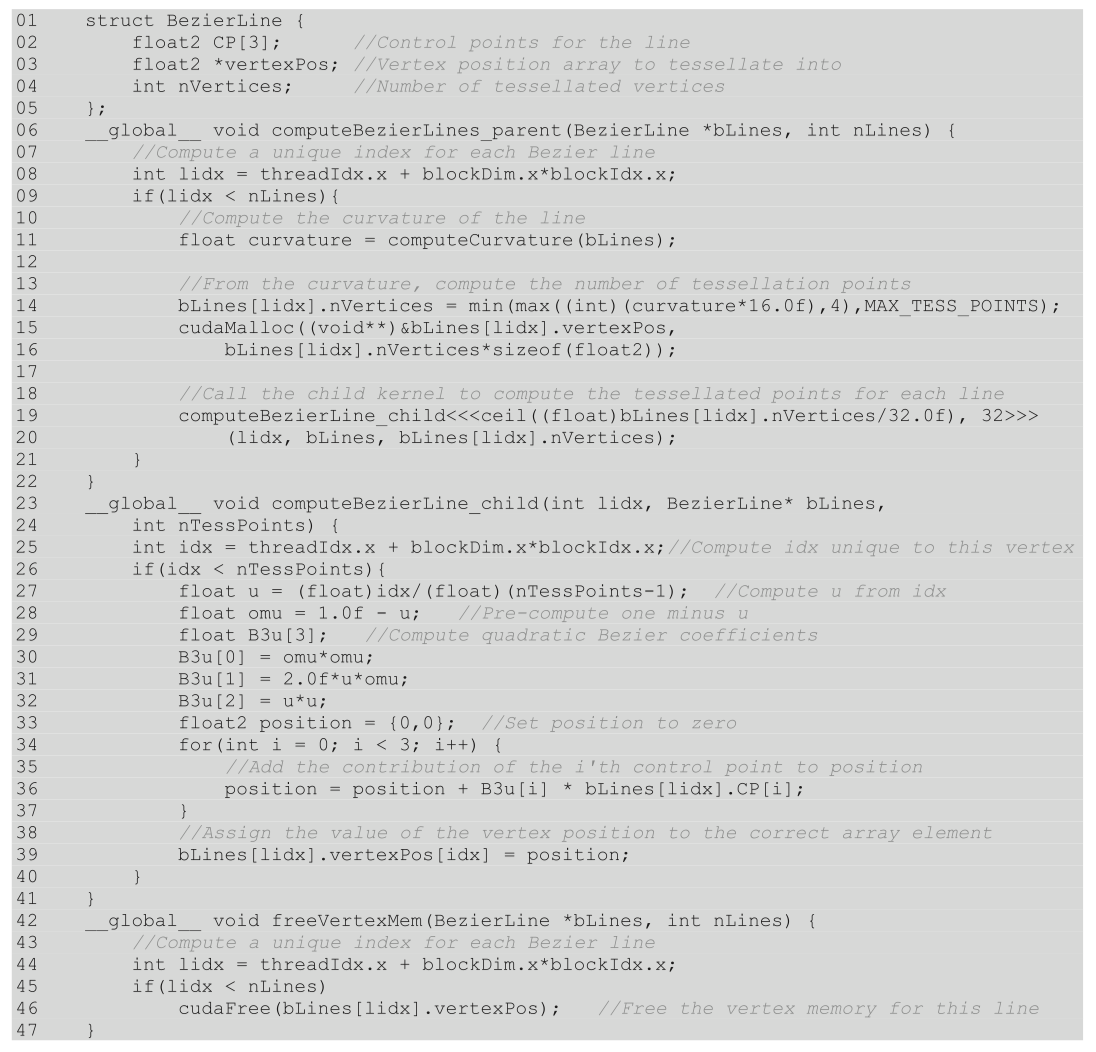
\includegraphics[width=0.9\textwidth]{figs/F21.7.png}
	\caption{\textit{可能的 SYCL 屏障死锁 }}
\end{figure}

在这种情况下,解决方法很简单:可以将范围检查移到 group\_barrier 之后,
或者在这种特定情况下,可以完全删除 group\_barrier。 
但情况并非总是如此,其他Kernel可能需要重组以确保所有Work-Items始终到达或始终跳过 group\_barrier。

\subsubsection{内存模型}
从根本上来说,CUDA 和 SYCL 都使用类似的弱有序内存模型。 
幸运的是,当我们将 CUDA Kernel迁移到 SYCL 时,我们只需要记住一些内存模型差异。

\paragraph{Barrier}

默认情况下,假设传递给 SYCL group\_barrier 的组是Work-Groups,
则 CUDA \_\_syncthreads Barrier函数和 SYCL group\_barrier Barrier函数对内存模型具有相同的效果。 
同样,假设传递给 SYCL group\_barrier 的组是Sub-Groups,
则 CUDA \_\_syncwarp Barrier函数与 SYCL group\_barrier Barrier函数具有相同的效果。

SYCL group\_barrier 接受一个可选参数来指定Barrier的 fence\_scope,但在大多数情况下,可以省略。 
可以将更广泛的范围传递给 group\_barrier,例如 memory\_scope::device,
但这通常不是必需的,并且可能会导致 SYCL group\_barrier 比 CUDA \_\_syncthreads Barrier更昂贵。

\begin{figure}[H]
	\centering
	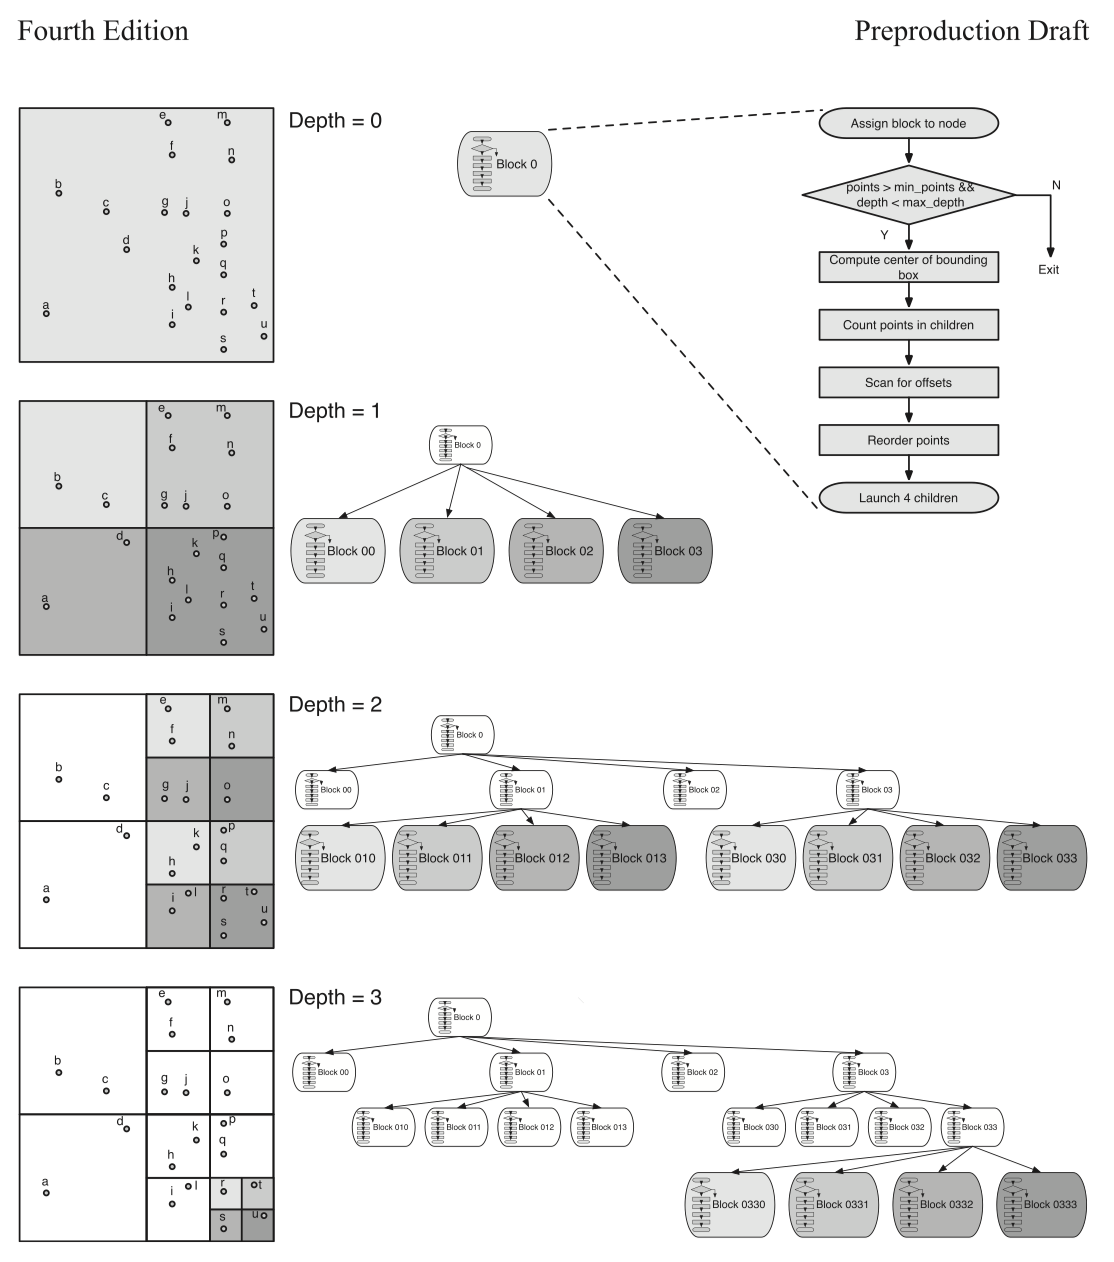
\includegraphics[width=0.9\textwidth]{figs/F21.8.png}
	\caption{\textit{CUDA 和 SYCL 的等效Barrier }}
\end{figure}

图 21-8 中的代码显示了 CUDA 和 SYCL 的等效Barrier语法。 
请注意,使用 this\_thread\_block 和 tiled\_partition 的较新 CUDA 协作组语法
如何具有更接近 SYCL group\_barrier 的同步函数。 
这是 CUDA 和 SYCL 2020 的后续版本变得越来越相似的另一个好例子。

\paragraph{原子和栅栏}

CUDA 和 SYCL 都支持类似的原子操作,尽管与Barrier一样,我们应该注意一些重要的差异。 
最重要的区别涉及默认的原子内存顺序。 
许多 CUDA 程序都是使用较旧的类似 C 的原子语法编写的,其中原子函数采用指向内存的指针,例如atomicAdd。 
这些原子函数是宽松的原子函数,并且在设备范围内运行。 
这些原子函数还有在不同作用域操作的后缀版本,
例如atomicAdd\_system 和atomicAdd\_block,但这些并不常见。

SYCL 原子语法有点不同,它基于 C++20 中的 std::atomic\_ref (
有关 SYCLatomic\_ref 类的详细信息以及它与 std::atomic\_ref 的比较,请参阅第 19 章)。 
如果我们希望 SYCLatomic 与 CUDAatomicAdd 函数等效,
我们需要声明 SYCLatomic\_ref 具有类似的 memory\_order::relaxed 内存顺序
和 memory\_scope::device 范围,如图 21-9 所示。

\begin{figure}[H]
	\centering
	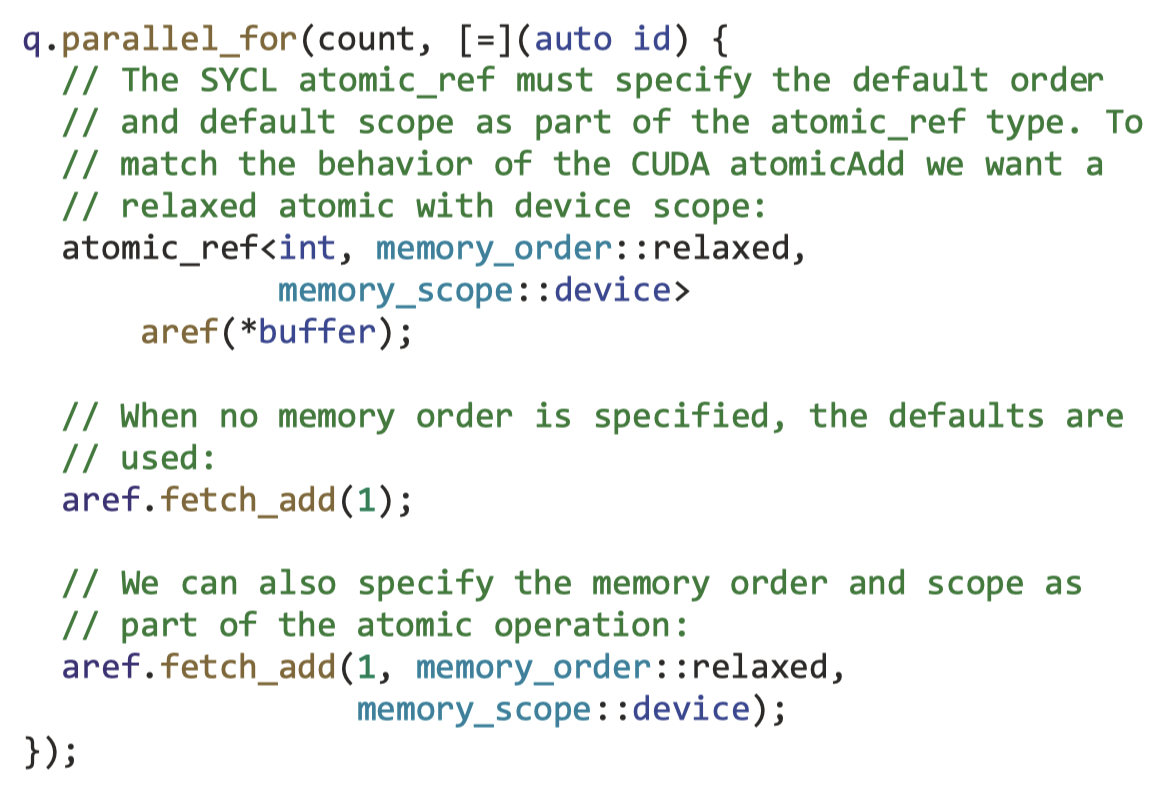
\includegraphics[width=0.9\textwidth]{figs/F21.9.png}
	\caption{\textit{CUDA 和 SYCL 等效原子操作 }}
\end{figure}

较新的 CUDA 代码可能使用 CUDA C++ 标准库中的 cuda::atomic\_ref 类。 
cuda::atomic\_ref 类看起来更像 SYCLatomic\_ref 类,但也有一些重要的区别需要注意:

\begin{itemize}
	\item CUDAatomic\_ref 的范围是可选的,但如果未指定,则默认为整个系统。 
在所有情况下,SYCLatomic\_ref 都必须指定原子范围。

	\item CUDAatomic\_ref 的默认原子顺序是无条件顺序一致性,
而SYCLatomic\_ref 可以指定不同的默认原子顺序。 
通过指定默认的原子顺序,我们的 SYCL 代码可以更加简洁,
并且即使原子顺序不是顺序一致性时也可以使用 += 等方便的运算符。
\end{itemize}

当我们的代码或算法需要原子时,我们需要记住最后一个问题:SYCL 规范不要求某些原子操作和原子范围,
并且可能并非所有 SYCL 设备都支持。 对于 CUDA 设备也是如此,但由于 SYCL 设备的多样性,记住 SYCL 尤为重要。 
有关如何查询 SYCL 设备属性的更多详细信息,请参阅第 12 章,
有关 SYCL 设备或上下文可能支持的原子功能的描述,请参阅第 19 章。

\subsubsection{其他差异}
本节介绍了将 CUDA 代码移植到 SYCL 时需要记住的一些其他差异。

\paragraph{项目类与内置变量}

CUDA 和 SYCL 之间较大的风格差异之一是Kernel实例识别其在 N 维并行索引空间中的位置的方式。 
回想一下第 4 章,每个 SYCL Kernel都必须采用一个项、一个 nd\_item、一个 id,
或者在某些情况下采用一个整数参数来标识并行索引空间中的Work-Items。 
item 和 nd\_item 类还可用于查询有关并行索引空间本身的信息,例如全局范围、局部范围以及Work-Items所属的不同组。

CUDA Kernel不包含任何参数来标识并行索引空间中的 CUDA 线程。 
相反,CUDA 线程使用内置变量(例如 blockIdx 和 threadIdx)来标识并行索引空间中的位置,
并使用内置变量(例如 gridDim 和 blockDim)来表示有关并行索引空间本身的信息。 
使用协作组的较新 CUDA Kernel还可以通过调用内置函数(如 this\_thread\_block)隐式构造某些协作组。

这通常只是一个语法差异,不会在功能上影响我们可以编写的代码,
尽管这确实意味着 SYCL Kernel在更多情况下可能会将一个项目或一个 nd\_item 传递给被调用函数,
例如被调用函数是否需要知道 work-item 索引。

\paragraph{上下文}

CUDA 和 SYCL 之间的另一个概念差异是 SYCL 上下文的概念。 
回想一下,SYCL 上下文是一个存储一组 SYCL 设备的 SYCL 应用程序状态的对象。 
例如,SYCL 上下文可以存储有关内存分配或编译程序的信息。 上下文对于 SYCL 应用程序来说是一个重要概念,
因为单个 SYCL 应用程序可能支持来自多个供应商的设备,可能使用多个后端 API。

在大多数情况下,我们的 SYCL 程序可能完全不知道上下文的存在,并且本书中的大多数示例程序都不会创建或操作上下文。 
如果我们确实选择在程序中创建额外的 SYCL 上下文(无论是隐式还是显式),
我们需要小心,不要将一个上下文中特定于上下文的 SYCL 对象与不同的 SYCL 上下文一起使用。 
充其量,不小心使用多个上下文可能会导致我们的程序运行效率低下,
比如说,如果我们最终多次编译 SYCL Kernel,每个上下文一次。 
在最坏的情况下,跨上下文混合 SYCL 对象可能会导致未定义的行为,导致我们的程序变得不可移植或在某些后端或设备上执行不正确。

为了完整起见,请注意 CUDA 也有上下文的概念,
尽管 CUDA 上下文仅由较低级别的 CUDA 驱动程序 API 公开。 大多数 CUDA 程序也不创建或操作上下文。

\paragraph{错误检查}

要考虑的最后一个区别与错误检查和错误处理有关。 
由于 CUDA 继承了 C 语言,CUDA 中的错误通过 CUDA 函数调用的错误代码返回。 
对于大多数 CUDA 函数,失败的错误代码表示返回错误的函数中存在错误,例如函数的参数不正确。 
但对于其他一些 CUDA 函数(例如 cudaDeviceSynchronize),错误值也可以返回设备上发生的异步错误。

SYCL 还具有同步和异步错误,尽管这两种类型的错误都是使用 SYCL 异常而不是 SYCL 函数的返回值来报告的。 
有关 SYCL 中错误检测和错误处理的更多信息,请参阅第 5 章。

\subsection{CUDA 中的功能尚未在 SYCL 中提供!}
到目前为止,我们已经描述了 CUDA 和 SYCL 中都有特征但表达方式不同的情况。 
本节介绍 CUDA 中的几个功能,但(当前)SYCL 中没有等效功能。 
这不是详尽的列表,但旨在描述 CUDA 应用程序常用的一些功能,这些功能在迁移到 SYCL 时可能需要更多努力。

请注意,供应商特定的功能是标准化过程的重要组成部分,无论它们是标准的扩展还是在完全供应商特定的 API 中定义。 
特定于供应商的功能提供了重要的实施经验,并允许功能在完善并纳入标准之前证明其价值。 
其中许多功能已经在积极开发中,以纳入 SYCL 标准,其中一些功能可能已经作为该标准的扩展提供。

\begin{remark}[参与进来!]
来自用户和开发人员的反馈是标准化过程的另一个重要部分。
如果您对新功能有想法,或者您发现其他 API 的扩展或功能很有价值,请考虑参与其中!
SYCL 是一个开放标准,许多 SYCL 实现都是开源的,因此可以轻松参与不断发展的 SYCL 社区。
\end{remark}

\subsubsection{全局变量}
尽管程序员很早就被告知永远不要使用全局变量,但有时全局变量是完成这项工作的正确工具。 
我们可能选择使用全局变量来存储有用的常量、查找表或我们希望执行数据并行Kernel的所有Work-Items都可以访问的其他值。

CUDA 支持不同地址空间中的全局变量,因此具有不同的生命周期。 
例如,CUDA 程序可以在全局内存空间中声明一个对于每个设备都是唯一的 \_\_device\_\_ 全局变量。 
这些全局变量可以由主机设置或从主机读取,并由执行Kernel的所有 CUDA 线程访问。 
CUDA 程序还可以在 CUDA 共享内存空间中声明一个 \_\_shared\_\_ 全局变量
(请记住,这相当于在 SYCL 本地内存中声明的变量),
该变量对于每个 CUDA 块都是唯一的,并且只能由该块中的 CUDA 线程访问 堵塞。

SYCL 尚不支持设备代码中的全局变量,尽管正在开发提供类似功能的扩展。

\subsubsection{协作组}
如本章前面所述,CUDA 的最新版本支持协作组,这为Barrier和洗牌函数等集体操作提供了替代语法。 
SYCL 组对象和 SYCL 组算法库与 CUDA 协作组有许多相似之处,但仍然存在一些关键差异。

最大的区别在于,SYCL 组功能目前仅适用于预定义的 SYCL Work-Groups和Sub-Groups类,而 CUDA 协作组则更加灵活。 
例如,CUDA 程序可以创建固定大小的tiled\_partition 组,
将现有组划分为一组更小的组,或者CUDA 程序可以将CUDA warp 中当前活动的CUDA 线程组表示为coalesced\_group。

CUDA 程序还可以创建比Work-Groups更大的协作组。 
例如,CUDA 程序可以创建表示网格中所有 CUDA 线程(相当于全局范围内的所有Work-Items)的 grid\_group,
或者表示线程块集群中所有 CUDA 线程的 cluster\_group。 
为了有效地使用这些更新和更大的组,必须使用特殊的主机 API 函数启动 CUDA Kernel,
以确保网格中的所有 CUDA 线程可以协作,或者指定线程块簇尺寸。

SYCL 尚不支持 CUDA 中的所有协作组类型,尽管正在进行扩展以向 SYCL 添加其他组类型。 
SYCL 2020 中引入的组对象和组算法使 SYCL 能够很好地支持此功能。

\subsubsection{矩阵乘法硬件}
我们将在本节中描述的最后一个功能是访问矩阵乘法硬件,也称为矩阵乘法和累加 (MMA) 硬件、张量核心或脉动阵列。 
这些都是专用硬件引擎的不同名称,这些引擎是专门为加速矩阵乘法运算而构建的,
而矩阵乘法运算对于许多人工智能 (AI) 工作负载至关重要。 
如果我们想要定制这些工作负载,那么必须能够访问数据并行Kernel中的矩阵乘法硬件以实现峰值性能,这一点非常重要。

CUDA 通过扭曲矩阵乘法和累加 (WMMA) 函数提供对矩阵乘法硬件的访问。 
这些函数有效地允许扭曲中的 CUDA 线程(相当于Sub-Groups中的Work-Items)协作以在较小的矩阵图块上执行矩阵乘法和累加操作。 
对于某些设备和算法,这些矩阵图块的元素可以是 32 位浮点型或 64 位双精度型,
但更常见的是使用较低精度的类型,例如 8 位字符、16 位半数或专用 AI 类型,例如 bfloat16s ( bf16)。

CUDA 和 SYCL 都在积极发展对矩阵乘法硬件的支持。 
这是一个很好的例子,说明不同的供应商最初如何通过特定于供应商的机制添加对其特定于供应商的功能的支持,
然后改进功能,并将常见的最佳实践添加到标准中。

\subsection{移植工具和技术}
幸运的是,当我们选择将应用程序从 CUDA 迁移到 SYCL 时,它不需要是手动过程,
我们可以使用工具来自动化部分迁移。 本节将介绍其中一种协助迁移的工具和技术。

\subsubsection{使用 dpct 和 SYCLomatic 迁移代码}
在本节中,我们将介绍 DPC++ 兼容性工具 (dpct) 和相关的开源 SYCLomatic 工具。 
我们将使用 dpct 自动将 CUDA 示例迁移到 SYCL,尽管本节中描述的概念同样适用于 SYCLomatic。

图 21-10 显示了我们将要迁移的简单 CUDA 示例的重要部分。 此示例反转缓冲区的块。 
这在实践中不是一个非常有用的示例,但它有我们的自动迁移工具需要处理的有趣情况,
例如 CUDA 共享内存全局变量、Barrier、设备查询、内存分配和初始化、Kernel调度本身, 以及一些基本的错误检查。

\begin{figure}[H]
	\centering
	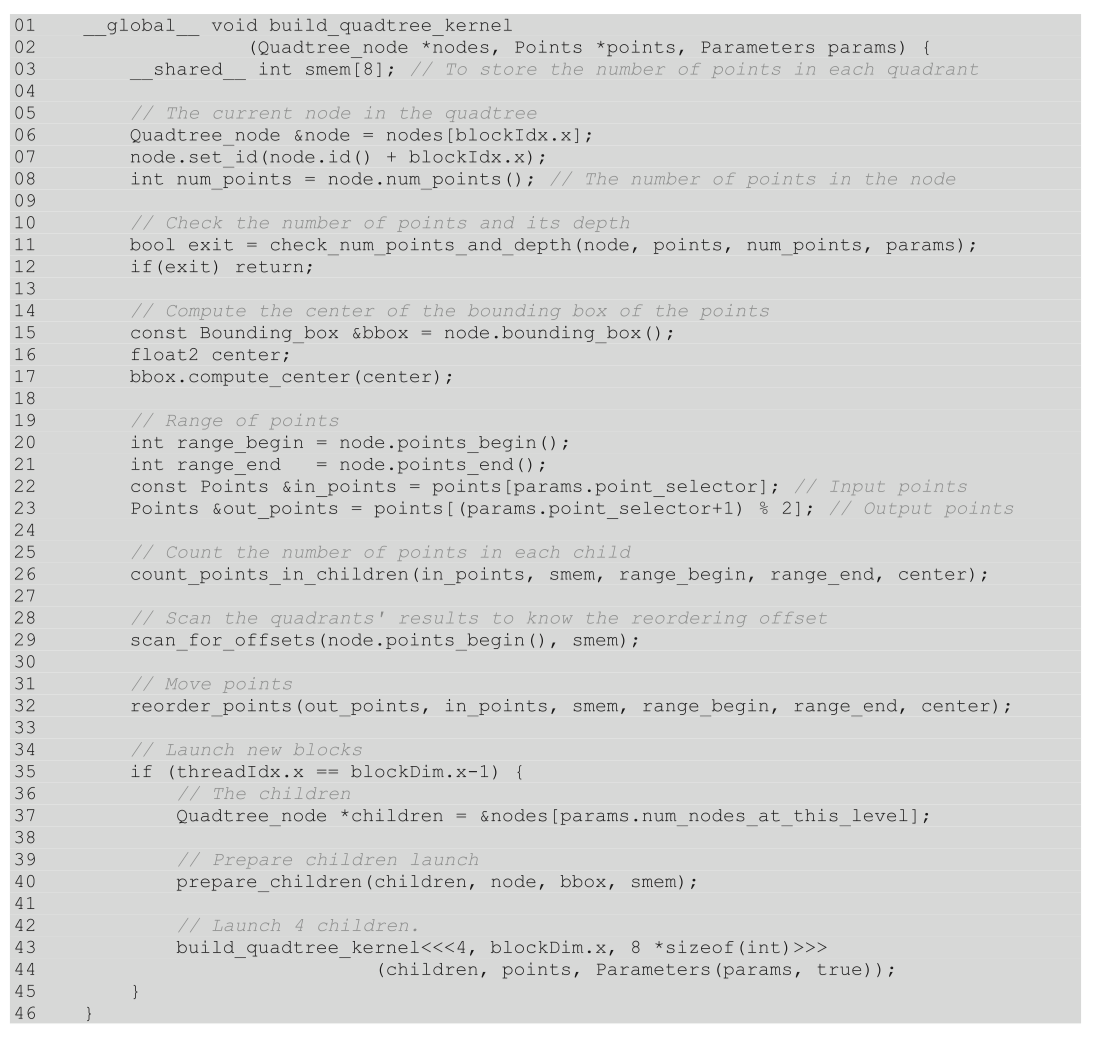
\includegraphics[width=0.9\textwidth]{figs/F21.10.png}
	\caption{\textit{我们将自动迁移一个简单的CUDA程序 }}
\end{figure}

\subsubsection{运行 dpct}

因为这是一个简单的示例,所以我们可以简单地调用 dpct 并传递我们想要迁移的 CUDA 源文件。 
对于更复杂的场景,可以在应用程序构建过程中调用 dpct 来识别要迁移的 CUDA 源文件。 
请参阅本章末尾的链接以获取更多信息和其他培训材料。

\begin{figure}[H]
	\centering
	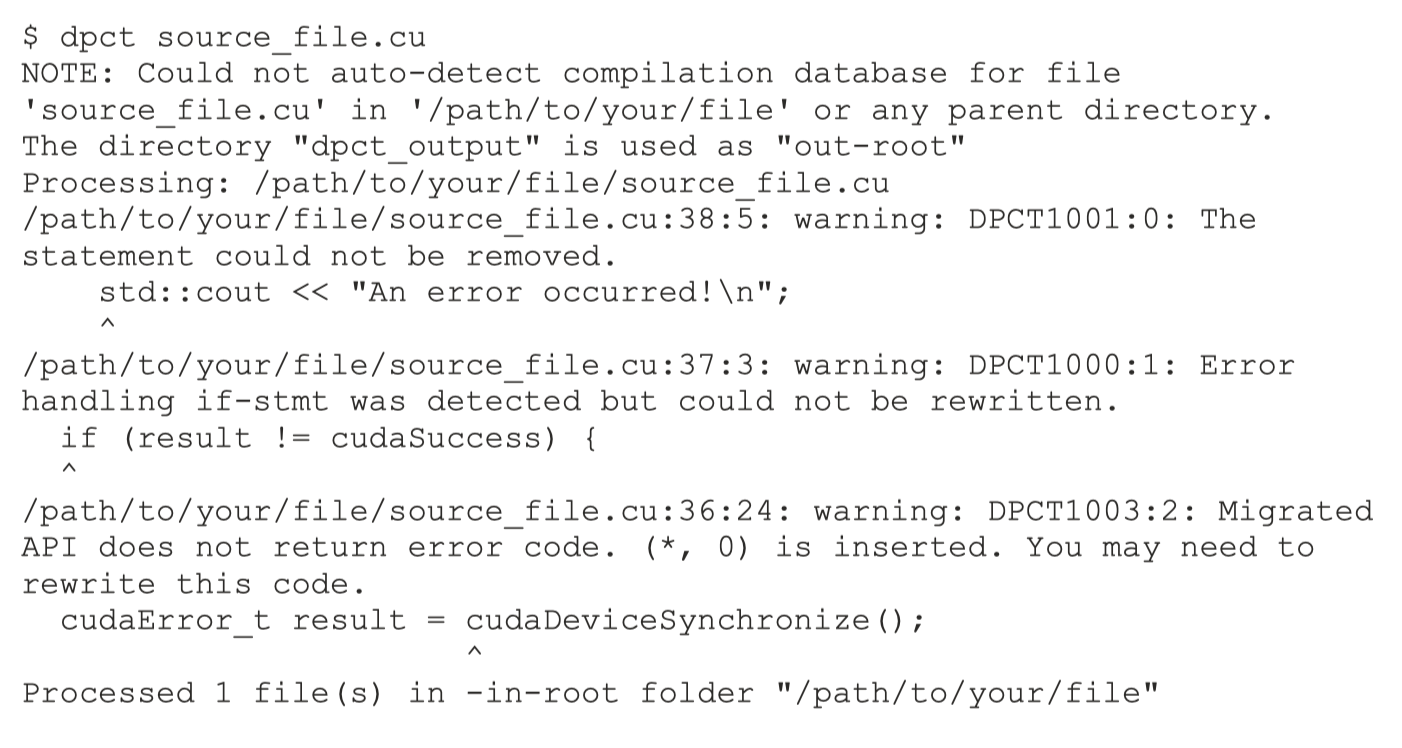
\includegraphics[width=0.9\textwidth]{figs/F21.11.png}
	\caption{\textit{迁移此 CUDA 程序时的示例 dpct 输出 }}
\end{figure}

当我们在示例 CUDA 源文件上运行 dpct 时,我们可能会看到如图 21-11 所示的输出。 
我们可以从这个输出中得出一些结论。 首先,我们的文件已成功处理,这太棒了! 不过,有一些警告表明 dpct 无法迁移。 
对于我们的示例,所有三个警告都是由于 CUDA 和 SYCL 之间的错误检查差异造成的。 
对于我们的程序,dpct 能够生成 SYCL 代码,当程序不生成错误时,该代码将正常运行,但它无法迁移错误检查。

错误检查警告是一个很好的例子,例如 dpct 和 SYCLomatic 等迁移工具将无法迁移所有内容。 
我们应该期望审查和调整迁移的代码以解决任何迁移问题,或者以其他方式改进迁移的 SYCL 代码的可维护性、可移植性或性能。

不过,对于此示例,我们可以按原样使用迁移的代码。

\begin{figure}[H]
	\centering
	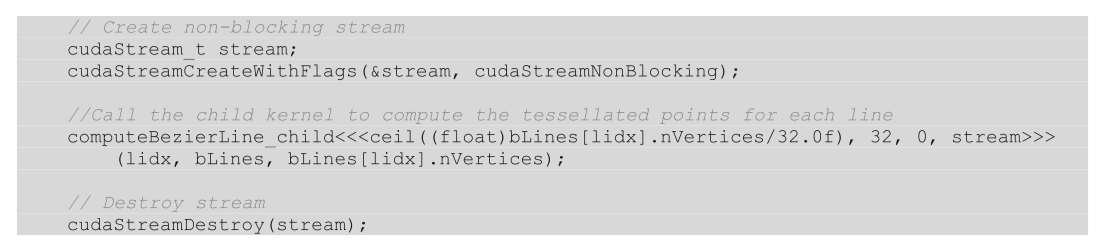
\includegraphics[width=0.9\textwidth]{figs/F21.12.png}
	\caption{\textit{编译和运行迁移的 CUDA 程序 }}
\end{figure}

图 21-12 显示了如何使用支持 NVIDIA GPU 的 DPC++ 编译器来编译迁移的代码,
然后显示我们的迁移程序在 Intel GPU、Intel CPU 和 NVIDIA GPU 上的成功执行。 
请注意,如果我们要在具有不同设备的不同系统上运行迁移的程序,
输出可能会有所不同,或者如果系统中不存在所选设备,则可能无法运行。

\subsubsection{检查 dpct 输出}

\begin{figure}[H]
	\centering
	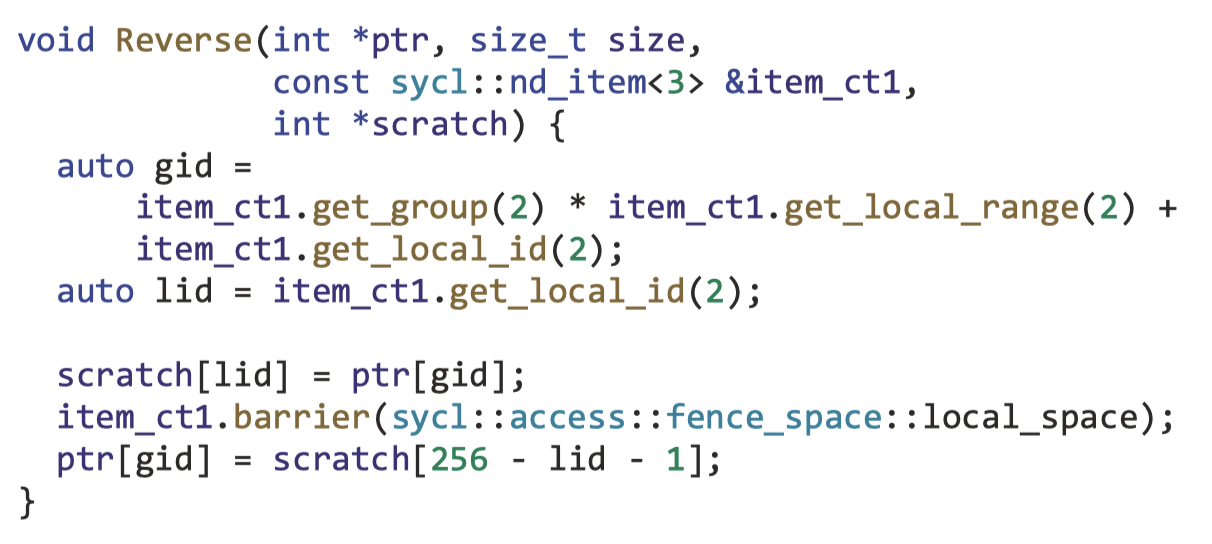
\includegraphics[width=0.9\textwidth]{figs/F21.13.png}
	\caption{\textit{从 CUDA 迁移的 SYCL Kernel }}
\end{figure}

如果我们检查迁移的输出,我们可以看到 dpct 处理了本章中描述的许多差异。 
例如,在图21-13所示的生成的SYCL Kernel中,
我们看到\_\_shared\_\_全局变量scratch被转换为本地内存访问器并传递到Kernel中。 
我们还可以看到,内置变量 blockIdx 和 threadIdx 被替换为对 nd\_item 类实例的调用,
并且连续维度的不同约定得到了正确处理,
例如,通过将 threadIdx.x 的使用替换为 调用 item\_gt1.get\_local\_id(2)。

\begin{figure}[H]
	\centering
	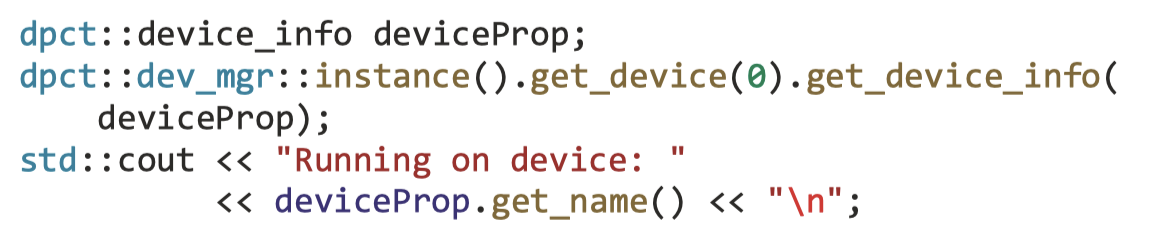
\includegraphics[width=0.9\textwidth]{figs/F21.14.png}
	\caption{\textit{从CUDA迁移的SYCL设备名称查询 }}
\end{figure}

我们还可以看到 dpct 通过使用几个 dpct 实用函数来处理一些主机代码差异,例如图 21-14 中所示的迁移设备查询。 
这些辅助函数仅供迁移后的代码使用。 为了可移植性和可维护性,我们应该更喜欢直接使用标准 SYCL API 进行额外的开发。

不过,总的来说,dpct 生成的 SYCL 代码是可读的,并且 CUDA 代码和迁移的 SYCL 代码之间的映射是清晰的。 
尽管通常需要额外的手动编辑,但使用 dpct 或 SYCLomatic 等自动化工具可以节省迁移过程中的时间并减少错误。

\subsection{总结}
在本章中,我们描述了如何将应用程序从 CUDA 迁移到 SYCL,
以使应用程序能够在任何 SYCL 设备上运行,包括使用支持 CUDA 的 SYCL 编译器的 CUDA 设备。

我们首先研究 CUDA 和 SYCL 程序之间的许多相似之处(抛开术语不谈)。 
我们看到了 CUDA 和 SYCL 如何从根本上使用相同的基于Kernel的并行方法,
以及相似的执行模型和内存模型,使得将 CUDA 程序迁移到 SYCL 相对简单。 
我们还探讨了 CUDA 和 SYCL 存在细微语法或行为差异的一些地方,
因此在我们将 CUDA 应用程序迁移到 SYCL 时最好记住这些差异。 
我们还描述了 CUDA 中但 SYCL 中尚未包含的几个功能(尚未!),
并且描述了特定于供应商的功能如何成为标准化过程的重要组成部分。

最后,我们研究了几种用于自动化部分迁移过程的工具,
并使用 dpct 工具将一个简单的 CUDA 示例自动迁移到 SYCL。 
我们看到了该工具如何自动迁移大部分代码,生成功能正确且可读的代码。 
迁移后,我们能够在不同的 SYCL 设备上运行迁移的 SYCL 示例,尽管更复杂的应用程序可能需要额外的检查和编辑。

\subsection{了解更多信息}
将 CUDA 代码迁移到 SYCL 是一个热门话题,还有许多其他资源可供了解更多信息。 作者发现以下两个有用的资源:

\begin{itemize}
	\item 显示如何从 CUDA 迁移到 SYCL 的一般信息和教程 (tinyurl.com/cuda2sycl)

	\item DPC++ 兼容性工具入门指南 (tinyurl.com/startDPCpp)
\end{itemize}